%%%%%%%%%%%%%%%%%%%%%%%%%%%%%%%%%%%%%%%%%%%%%%%%%%%%%%%%%%%%%%%%%%%%%%
% Overleaf (WriteLaTeX) Example: Molecular Chemistry Presentation
%
% Source: http://www.overleaf.com
%
% In these slides we show how Overleaf can be used with standard 
% chemistry packages to easily create professional presentations.
% 
% Feel free to distribute this example, but please keep the referral
% to overleaf.com
% 
%%%%%%%%%%%%%%%%%%%%%%%%%%%%%%%%%%%%%%%%%%%%%%%%%%%%%%%%%%%%%%%%%%%%%%
% How to use Overleaf: 
%
% You edit the source code here on the left, and the preview on the
% right shows you the result within a few seconds.
%
% Bookmark this page and share the URL with your co-authors. They can
% edit at the same time!
%
% You can upload figures, bibliographies, custom classes and
% styles using the files menu.
%
% If you're new to LaTeX, the wikibook is a great place to start:
% http://en.wikibooks.org/wiki/LaTeX
%
%%%%%%%%%%%%%%%%%%%%%%%%%%%%%%%%%%%%%%%%%%%%%%%%%%%%%%%%%%%%%%%%%%%%%%

\documentclass{beamer}

% For more themes, color themes and font themes, see:
% http://deic.uab.es/~iblanes/beamer_gallery/index_by_theme.html
%
\mode<presentation>
{
  \usetheme{Madrid}       % or try default, Darmstadt, Warsaw, ...
  \usecolortheme{default} % or try albatross, beaver, crane, ...
  \usefonttheme{serif}    % or try default, structurebold, ...
  \setbeamertemplate{navigation symbols}{}
  \setbeamertemplate{caption}[numbered]
} 

\usepackage[english]{babel}
\usepackage[utf8x]{inputenc}
\usepackage{chemfig}
\usepackage[version=3]{mhchem}

% On Overleaf, these lines give you sharper preview images.
% You might want to `comment them out before you export, though.
\usepackage{pgfpages}
\pgfpagesuselayout{resize to}[%
  physical paper width=8in, physical paper height=6in]

%==================================
\usepackage{subfigure}
\usepackage[]{algorithm2e}
%\usepackage{algorithm}
%\usepackage{algorithmic}

% \REDCOMMENT{text}
\newcommand{\REDCOMMENT}[1]{\color{red}{#1}\color{black}}

% \BLUECOMMENT{text}
\newcommand{\BLUECOMMENT}[1]{\color{blue}{#1}\color{black}}

%==================================

% Here's where the presentation starts, with the info for the title slide
\title[My Computer Graphics Background]{A presentation on my background in computer graphics}
\author{M. Mostajab}
\institute{www.mmostajab.com}
\date{\today}

\begin{document}

\begin{frame}
  \titlepage
\end{frame}

% These three lines create an automatically generated table of contents.
\begin{frame}{Outline}
  \tableofcontents
\end{frame}

\section{Introduction}

\begin{frame}{About Me...}
	\begin{tikzpicture}[overlay, remember picture]
		\node[anchor=north east, xshift=-30pt,yshift=-55pt]
		at(current page.north east){
			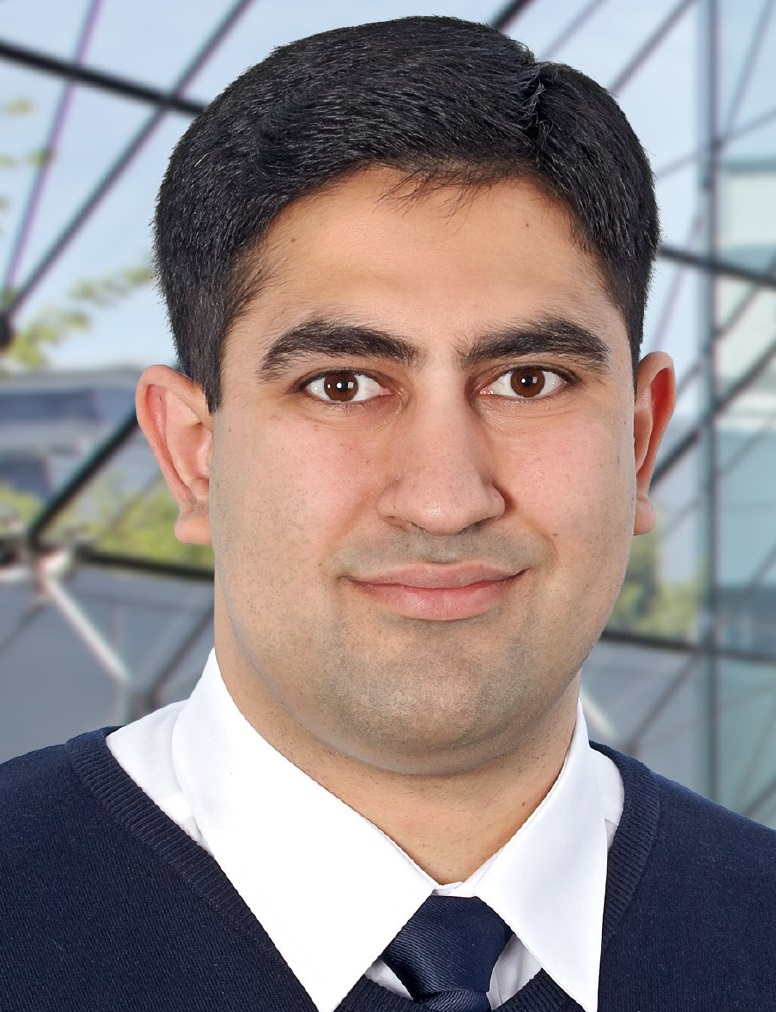
\includegraphics[width=30mm]{figures/photo.jpg}
		};
	\end{tikzpicture}

	\begin{itemize}
		\item My name is \textbf{Morteza Mostajab}
		\item Bachelor studies:\\ \textit{Hamedan University of Technology, Iran}
		\item Maseter studies:\\ \textit{Technische Universit{\"a}t M{\"unchen}}
		\item Present:\\ \textit{Researcher at Fraunhofer IGD, Darmstadt}
		\item Research interests:\\
		    \textit{Real-time physically-based rendering} \\
			\textit{(Rasterization-based or Ray-tracing)}\\
			\textit{Virtual reality}\\
			\textit{Computer graphics and visualization}\\
			\textit{Game Programming}
		   
	\end{itemize}
\end{frame}

\begin{frame}{Inspiration}
	
	\begin{itemize}
		\item Games, Animations, Movies with Special Effects,...
			\begin{figure}
			\centering
			\subfigure[Last Ninja 3]{
				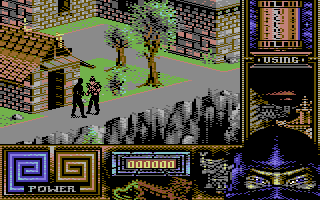
\includegraphics[width=0.19\linewidth]{figures/LastNinja.png}
			}
			%\subfigure[Warcraft 2]{
			%	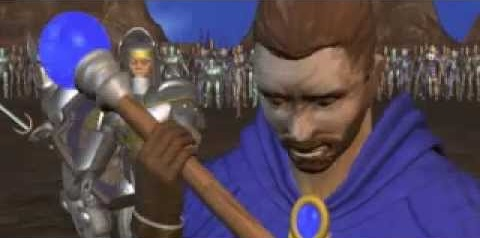
\includegraphics[width=0.2\linewidth]{figures/warcraft2.jpg}
			%}
			\subfigure[Gears of War]{
				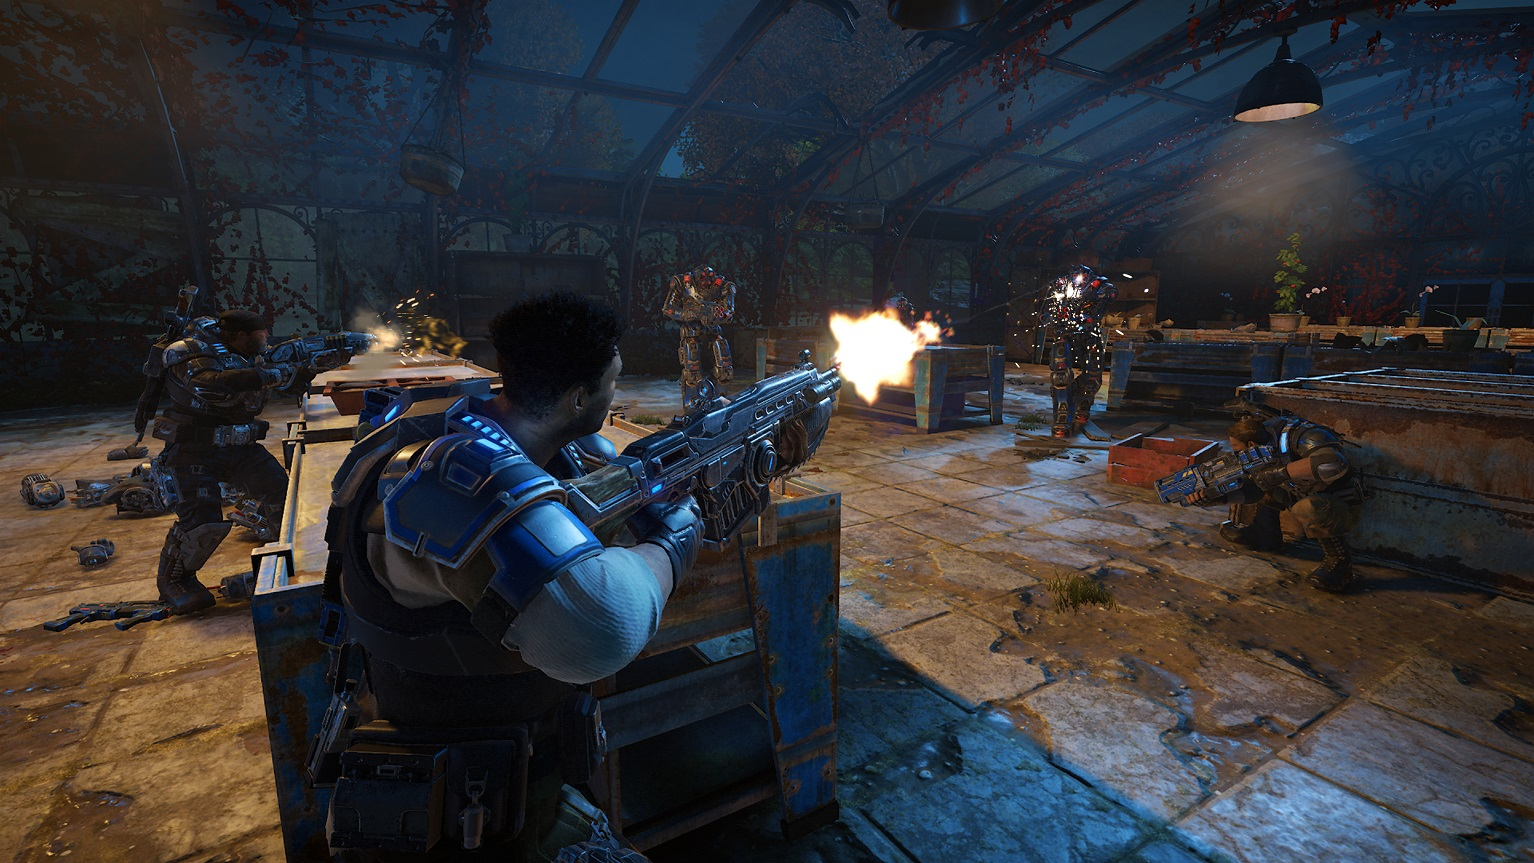
\includegraphics[width=0.21\linewidth]{figures/geow.jpg}
			}
			\subfigure[Ratatouille]{
				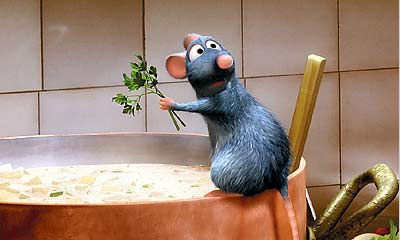
\includegraphics[width=0.20\linewidth]{figures/Ratatouille.jpg}
			}
			\subfigure[The lord of the rings]{
				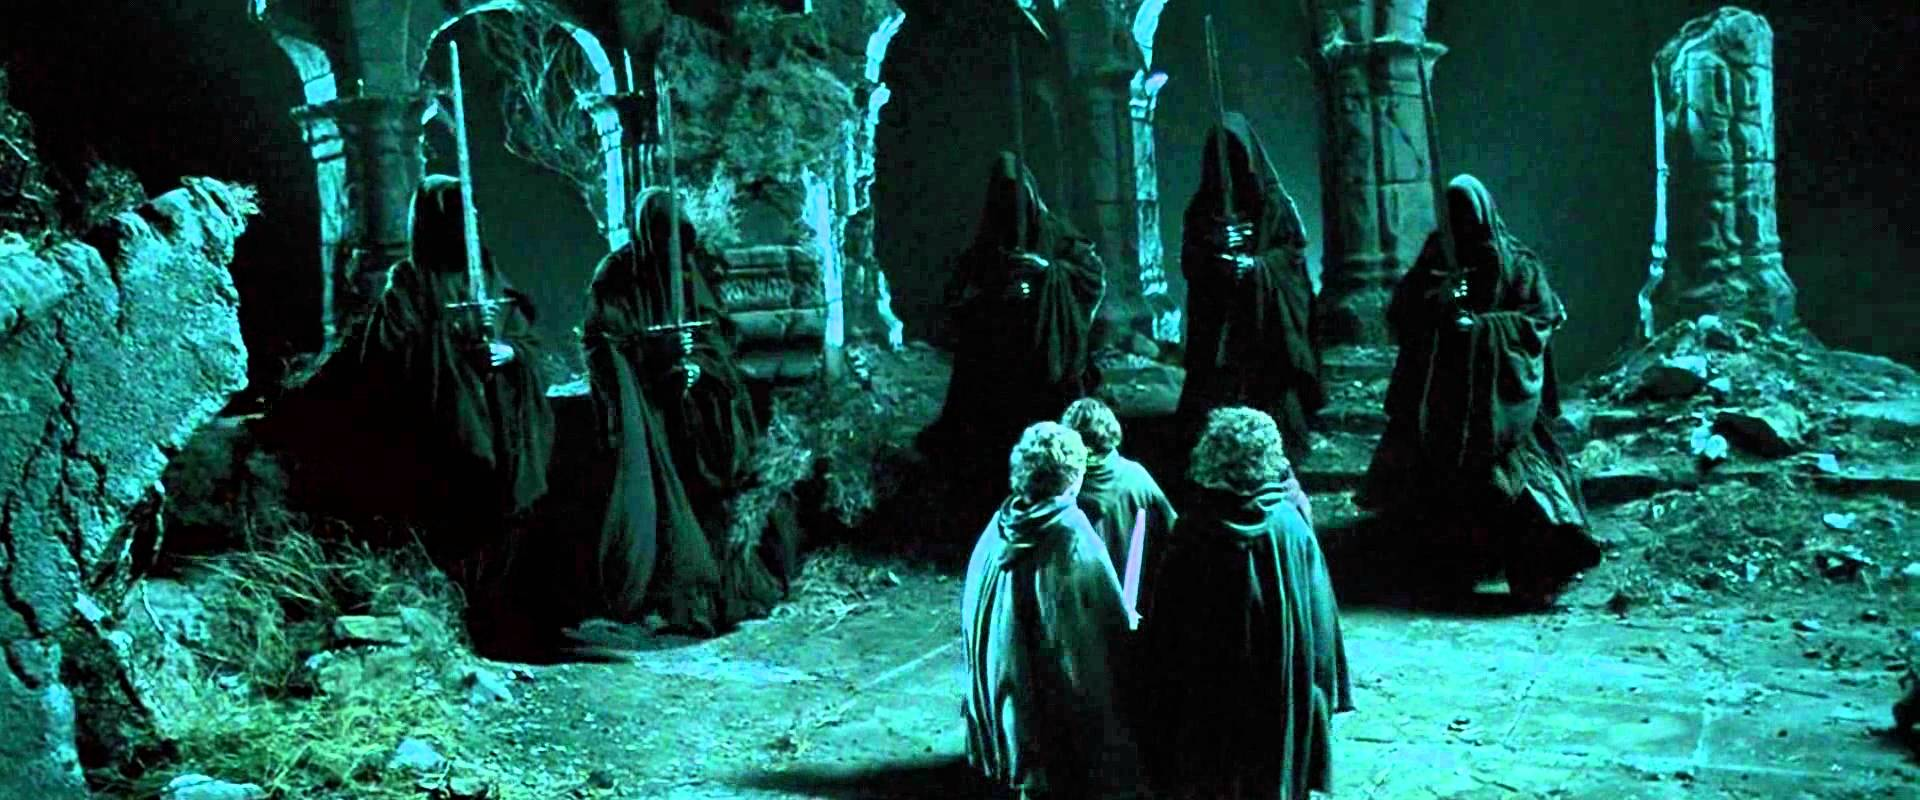
\includegraphics[width=0.29\linewidth]{figures/lotr.jpg}
			}		
		\end{figure}
	  \item My firsts...
		  \begin{figure}
			\centering
			\subfigure[First Computer]{
				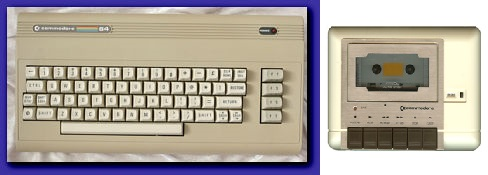
\includegraphics[height=0.2\textheight]{figures/commodore.jpg}
			}
			\subfigure[First IBM compatiable PC]{
				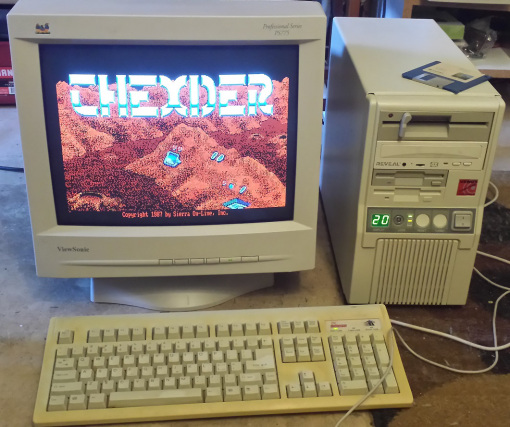
\includegraphics[height=0.2\textheight]{figures/PC286.jpg}
			}
			\subfigure[First Console (Atari 2600)]{
				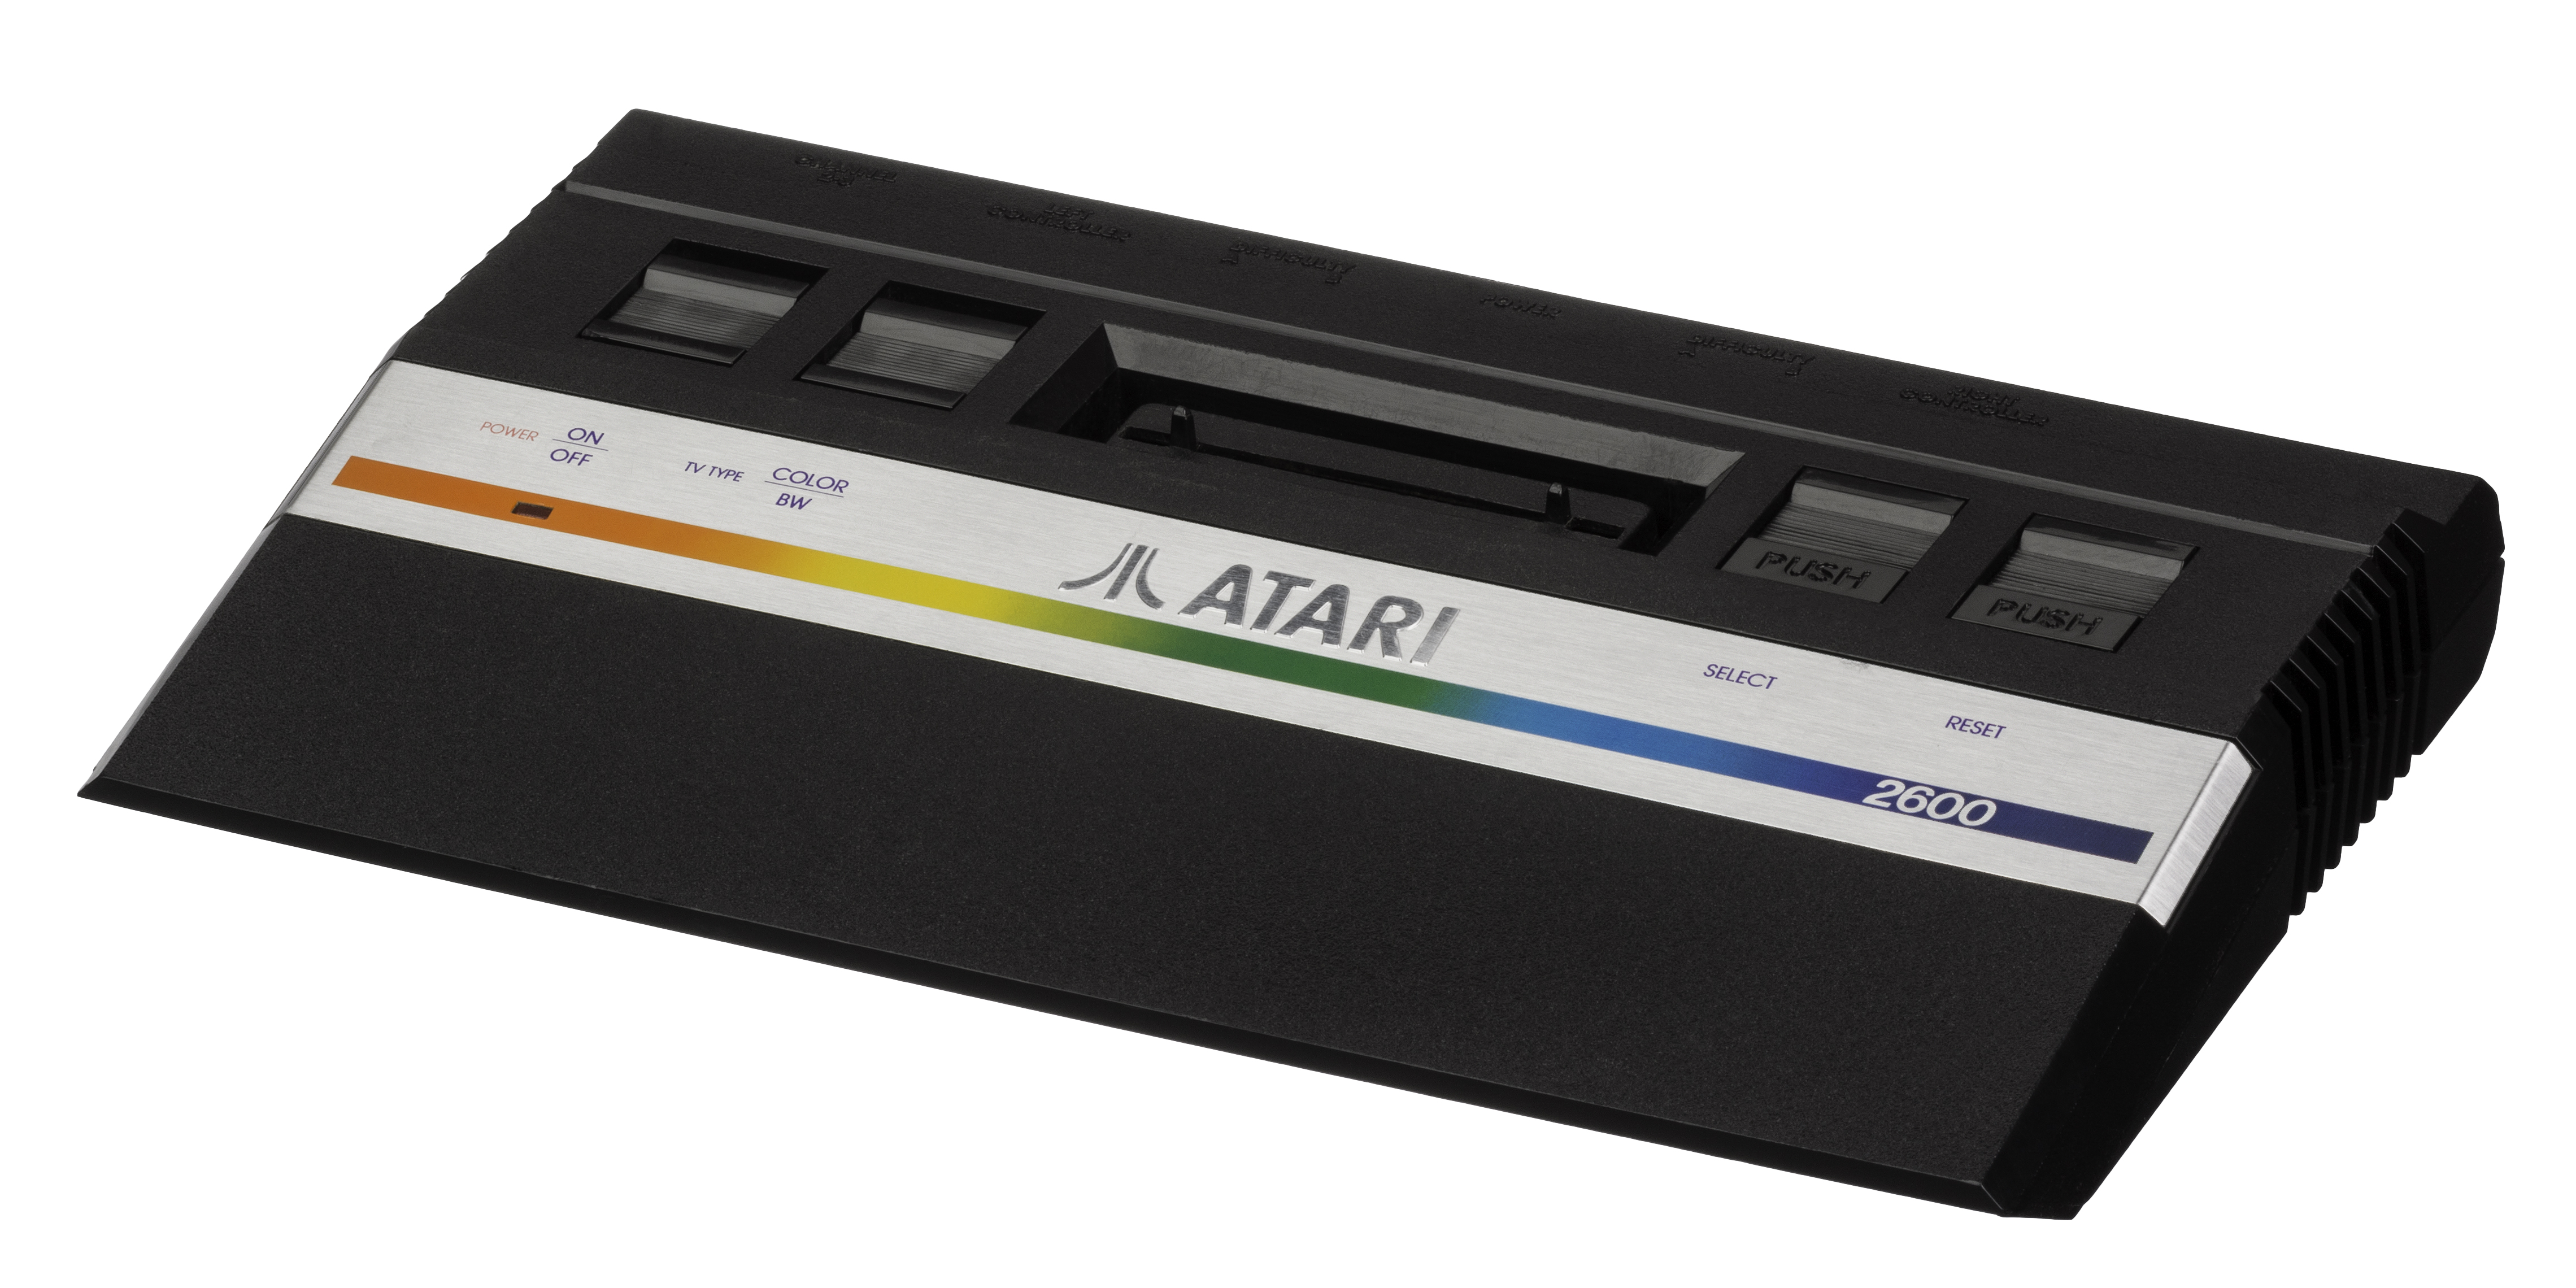
\includegraphics[height=0.15\textheight]{figures/atari2600.jpg}
			}
       	  \end{figure} 
	\end{itemize}
\end{frame}

\begin{frame}{Outline}
	\tableofcontents
\end{frame}

\section{Master Thesis}

\begin{frame}{Motivation}
	\begin{itemize}
		\item \textbf{Goal}: Use virtual reality to help engineers getting a better \textbf{understanding} of simulations, make \textbf{investigation} in flow field features easier.
		\item Virtual reality applications demands 75-140 frames per second scene update and rendering to reduce \textbf{latency}.
		\item \textbf{Initial motivation}:\\
		  -- \textbf{Immersive Streamline Demo}: a demo which user could stand in a simulation model to understand flow field features by:
		  \begin{itemize}
		  	\item Prototype demo which placed the user virtually in simulation model.
		  	\item User could interact with virtual world by moving streamlines' seeding plane.
		  	\item User could walk around in the simulation model, look closer into streamlines to understand flow field's features better.
		  \end{itemize} 
	\end{itemize}
\end{frame}

\begin{frame}{Immersive Streamline Demo}

	\begin{figure}[ht!]
	\centering
	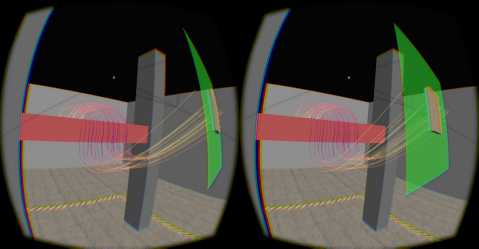
\includegraphics[width=0.9\linewidth]{./figures/vr.png}
	\caption{\textbf{Immersive Streamlines} was a prototype demo done at Fraunhofer IGD. The user is able to move inside the virtual world, interact with it, and look closely at the flow visualization results. The image shows a stereo pair, which is displayed on Oculus Rift HMD. }
	\label{fig:vr_irpv}
	
	\end{figure}
\end{frame}

\begin{frame}{Problem Definition}
	\begin{itemize}
		\item Streamline's computation was 10 frames per second (latency was very visible to user).
		\item Streamline's accuracy was not high enough (straight lines in streamlines are visible in the screenshot).
		\item Stream surfaces can provide more information about flow fields features.
		\item So, we defined \textbf{Parallel Stream Surface Computation and Rendering} master thesis to solve these problems.		
	\end{itemize}
\end{frame}

\begin{frame}{Main Contributions}
	\begin{itemize}
		\item Investigation techniques from ray tracing field for application in accurate streamline computation:\\
		  -- Using acceleration structures\\
		  -- Using ray-packing\\
		\item Using heterogeneous computing:\\
		  -- Scale streamline computation on all capable devices.\\
		  -- Scale rendering on all graphic processing units.\\
	\end{itemize}
\end{frame}

\begin{frame}{Benefits}
	
	\begin{itemize}
		\item Accurate streamline computation method (using \textbf{Runge-Kutta} integration method).
		\item \textbf{Adaptive Runge-Kutta} integration method to adapt steps to maximum integration error.
		\item Heterogeneous stream surface computation.
		\item Multi GPU stream surface computation and result 
	\end{itemize}
	\textbf{}
	
\end{frame}

\begin{frame}{Related Works}
	\begin{itemize}
		\item Parallel stream surface computation for large data sets \cite{CampPaper}.\\
		proposed a distributed stream surface computation system.\\
		-- \textbf{My method is not distributed but uses all available computation devices.}
		\item Interactive Streak Surface Visualization on the GPU \cite{BurgerStreakSurface}.\\
		Bue+09 samples the simulation mesh on a regular grid, then compute the streak surface.\\
		-- \textbf{Reduces accuracy, ignores a lot of information exist in simulation mesh by sampling it on a regular grid.}
	\end{itemize}
\end{frame}

\begin{frame}{Related Works}
	\begin{itemize}
		\item Interactive particle tracing for the exploration of flow fields in virtual environments \cite{Schirski:50085}.\\
		Sch08 uses the neighboring graph instead of acceleration
		structure on GPU.\\
		-- \textbf{step size needed to be small enough.}
		\item Fast, Memory-Efficient Cell Location in Unstructured Grids for
		Visualization \cite{GarthPaper}.\\
		introduces cell-tree acceleration structure use it for
		particle tracing.\\
		-- \textbf{I have evaluated more acceleration structures to classify them based on memory requirements and performance.}
	\end{itemize}
\end{frame}

\begin{frame}{Stream Surface Computation Algorithm \cite{CampPaper}}
	\begin{algorithm}[H]
		\KwData{$seeds$ list which contains all initial seeding points.}
		\KwResult{Stream Surface Points}

		\While{$seeds$ list is not empty}{
			
			\textbf{Tracing}: Trace streamlines originating from seeding points stored in $seeds$ list.\
			
			\textbf{Refinement}:\For{each pair of adjacent streamlines $s_1$ and $s_2$}{
		$d \gets$ \textit{Distance}($s_1$, $s_2$)\
		
				\eIf{$d \leq D_{disc}$ }{
					\textbf{Discontinuity}: The surface is discontinued in that area.
				}{
					$s_{new} \gets (s_1[0] + s_2[0]) / 2$\\			  
					add $s_{new}$ to list $seeds$.
				}
			}
		}
		\caption{Stream Surface Computation Algorithm \cite{CampPaper}.}
	\end{algorithm}
\end{frame}

\begin{frame}{Accurate Streamline Computation}
	\begin{itemize}
		\item Point-Inside-Cell checks \& interpolating results inside cells.
		\item Using \textit{adaptive Runge-Kutta} integration method (Cash-Karp).
		\item Adaptive stepping (faster and more accurate integration).
		\item Avoiding early terminations.
	\end{itemize}
    \begin{figure}
    	\centering
    	\subfigure[Euler]{
    		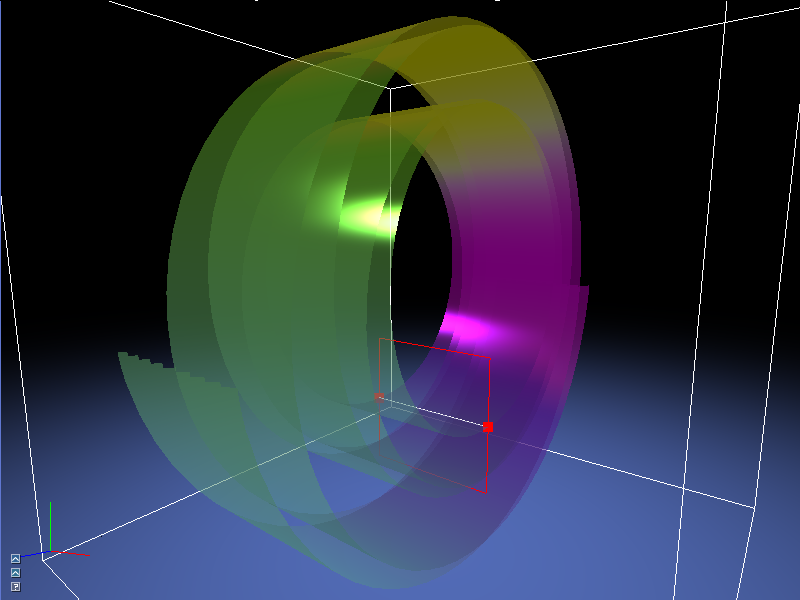
\includegraphics[width=0.4\linewidth]{figures/euler}
    	}
    	\subfigure[Cash-Karp]{
    		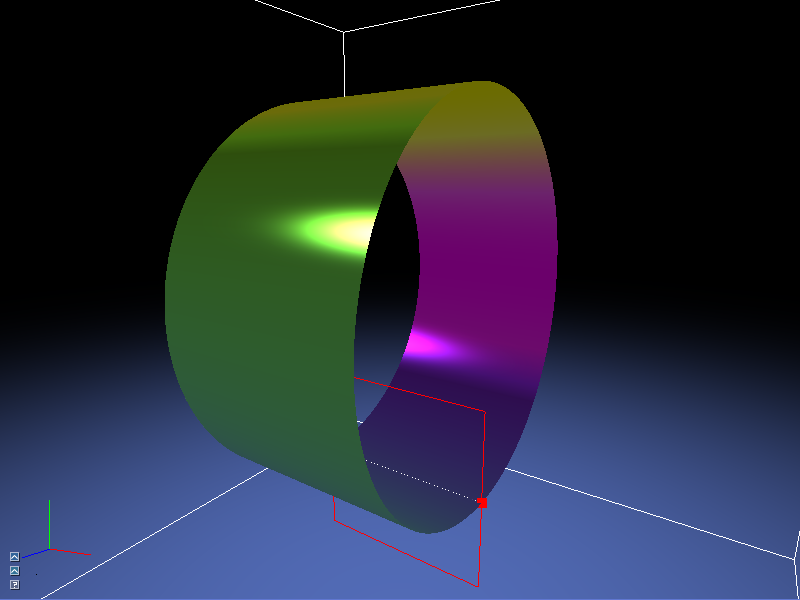
\includegraphics[width=0.4\linewidth]{figures/cashkarp}
    	}
	    \caption{Euler and Runge-Kutta integration methods in a perfect rotation around center which are integrated with the same step size.}
    \end{figure}
\end{frame}

\begin{frame}{Refinement Strategy Results}
	\begin{figure}
		\centering
		\subfigure[No Refinements]{
			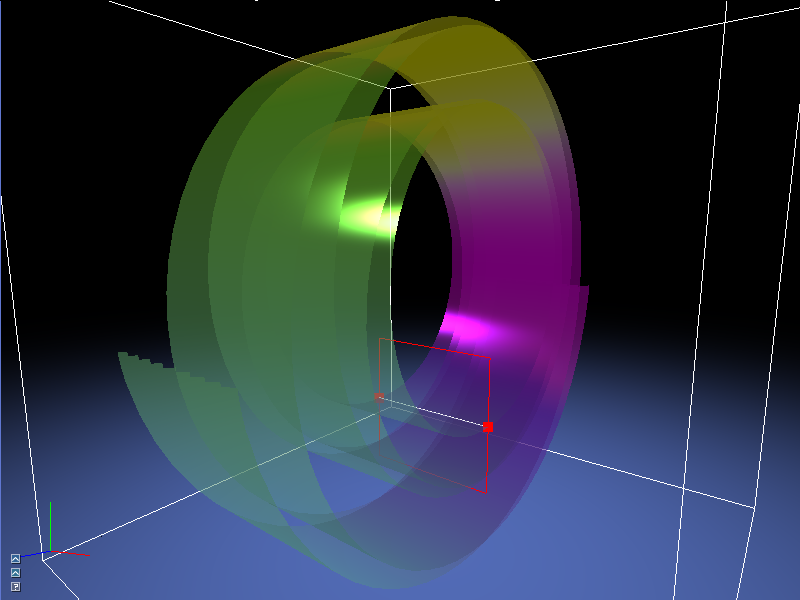
\includegraphics[width=0.3\linewidth]{figures/euler}
		}
		\subfigure[The first refinement iteration]{
			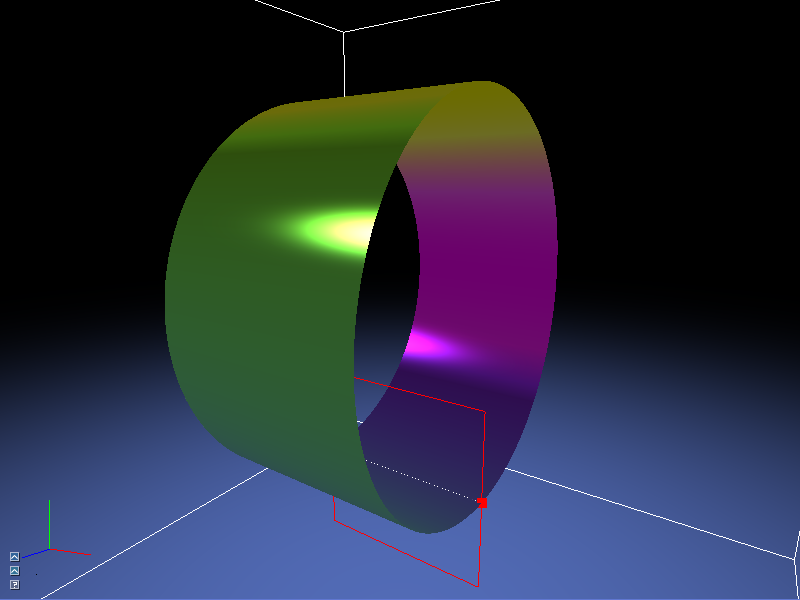
\includegraphics[width=0.3\linewidth]{figures/cashkarp}
		}
		\subfigure[The second refinement iteration]{
			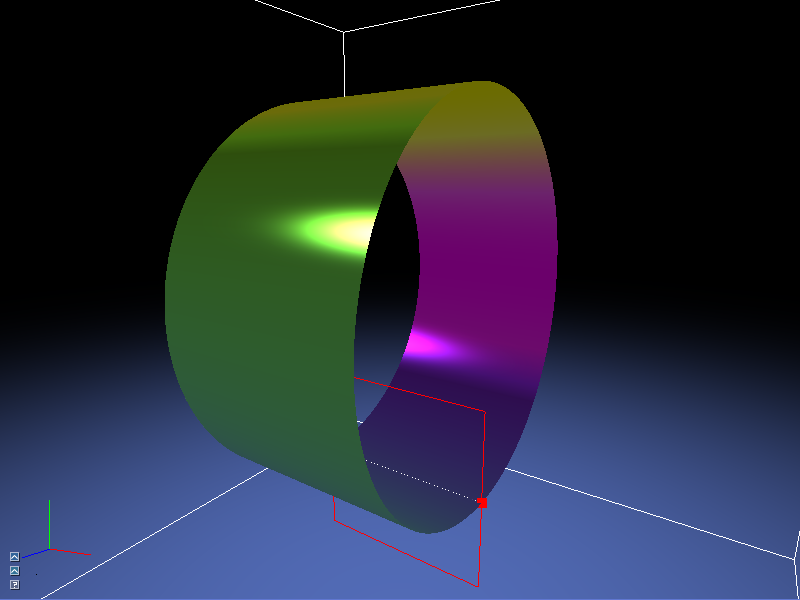
\includegraphics[width=0.3\linewidth]{figures/cashkarp}
		}
		\caption{The result streamlines making skeleton of stream surface after 2 steps refinement.}
	\end{figure}
\end{frame}

\begin{frame}{Heterogeneous computing model}
	What was in my thesis.
\end{frame}

\begin{frame}{Static Distribution of Seeding Points}
	What was in my thesis.
\end{frame}

\begin{frame}{Dynamic Distribution of Seeding Points}
	What will be implemented in holidays 2016.
\end{frame}

\begin{frame}{Heterogeneous computing results}
	What I will measure.
\end{frame}

\begin{frame}{Acceleration Structures}
	\begin{itemize}
		\item Grid
		\item Kd-tree
		\item Bounding Volume Hierarchy (BVH)
		\item Cell-tree \cite{GarthPaper}
	\end{itemize}

	\begin{figure}[!ht]
		\centering
		
		
		\caption{method}
	\end{figure}

\end{frame}

\begin{frame}{Why Acceleration Structures?}
	\begin{itemize}
		\item Accelerating cell look up for faster streamline computation.
		\item Ray tracing uses acceleration structures to find \textbf{nearest intersection point} in contrast to streamline computation which uses it to \textbf{sample result in a specific point}.
		\item Differences:
		    \begin{itemize}
		    	\item In streamline computation instead of \textit{Surface Area} Heuristics, textit{Volume} Heuristics should be used.
		    	\item \textit{Traversal algorithms} for space partitioning cases does not need \textit{stack}.
		    	\item Hierarchy traversal algorithms need a greedy method to prefer one child to other one during traversal.
		    \end{itemize}
		
	\end{itemize}
\end{frame}

\begin{frame}{Acceleration Structures Comparison Results}
	\begin{itemize}
		\item The origin...
	\end{itemize}
\end{frame}

%================================================
%================================================

\section{Ray tracing revisited for rendering CSG models consisting of higher order primitives}

\begin{frame}{Outline}
	\tableofcontents
\end{frame}

\begin{frame}{Ray tracing revisited for rendering CSG models consisting of higher order primitives}
	\begin{figure}[ht!]
		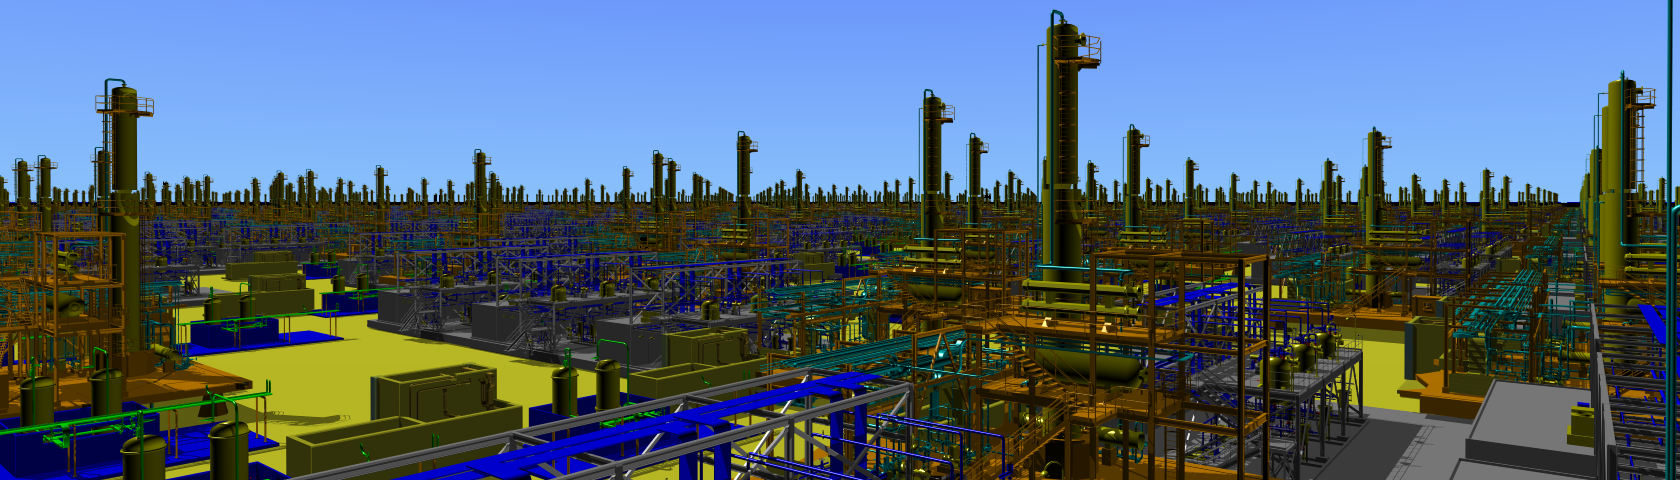
\includegraphics[width=1.0\linewidth]{figures/Plant_Teaser.png}
		\caption{
			A complex CAD scene built out of 8,000 individual plant models. In total, the scene consists of more than 100,000,000 non-planar second-order (cylinders, cones, etc.) and forth-order (tori) primitives, ray traced at more than 10~frames per second on 16 CPU
			cores, including pixel-accurate shadows.
		}
	\end{figure}
\end{frame}

\begin{frame}{Benefits}
	\begin{itemize}
		\item \textbf{On-the-fly compositing.}\\
		%
		-- Boolean set operations are performed on a per-ray basis immediately	during rendering.\\
		-- No Preprocessing.
		\item \textbf{Low storage requirement.}\\
		%
		-- small set of parameters for each primitive.\\
		-- No prior triangulation of primitives.
		-- Holding scenes in memory would be possible without triangulation.
		\item \textbf{Pixel-accurate higher order surfaces.}\\
		-- Ray-primitive intersection can be tested directly.
		-- Usually a quadratic equation which is easy to solve (tori has a quartic equation).\\
		-- No discretization artifacts are visible.\\
		-- Surfaces appear perfectly smooth.\\
	\end{itemize}
\end{frame}

\begin{frame}{Main Contributions}
	\begin{itemize}
		\item a method to apply CSG operations in real-time during ray tracing while keeping the memory overhead low.
		\item Evaluation of the proposed method in comparison to other well-known rasterization-based real-time CSG model rendering techniques(\cite{goldfeather:86:FCSGDPPGS}, and \cite{Stewart02linear-timecsg}).
	\end{itemize}
\end{frame}

\begin{frame}{Optimized Hitpoint Calculation}
	\begin{algorithm}[H]
		\BLUECOMMENT {$ray$: current ray hitting a primitive}\\
		\vspace{0.5mm}
			\eIf{ entering primitive }
			{ $delta$ := $+1$; }
			{ $delta$ := $-1$; }

			\eIf{ positive primitive hit }
			{ $ray.posDepth$ += delta;  }
			{ $ray.negDepth$ += delta;  }

			\eIf{ ($ray.posDepth>0$) $\&\&$ ($ray.negDepth<=0$) }
			{ ReportHit(); \BLUECOMMENT{ // final hit in layer found } }
			{ ContinueRay($ray$); \BLUECOMMENT{ // still inside a negative medium } }		
		\caption{RayTraceLayer($ray$)}
		\label{alg:ray-trace-layer}
	\end{algorithm}
\end{frame}

\begin{frame}{Supported Higher order primitives}
	
	\begin{figure}[ht!]
		\centering
		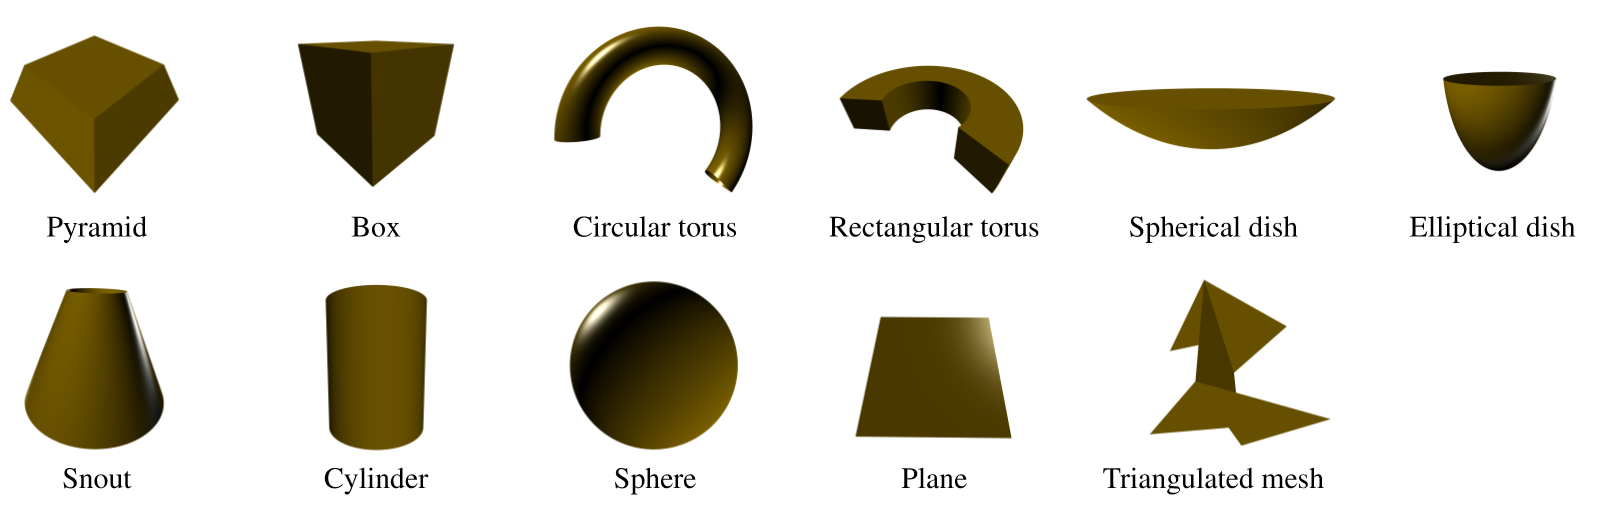
\includegraphics[width=0.9\linewidth]{figures/hops.png}
	\end{figure}
\end{frame}

\begin{frame}{More Results}	
	\begin{figure}
		\centering
		\subfigure{
			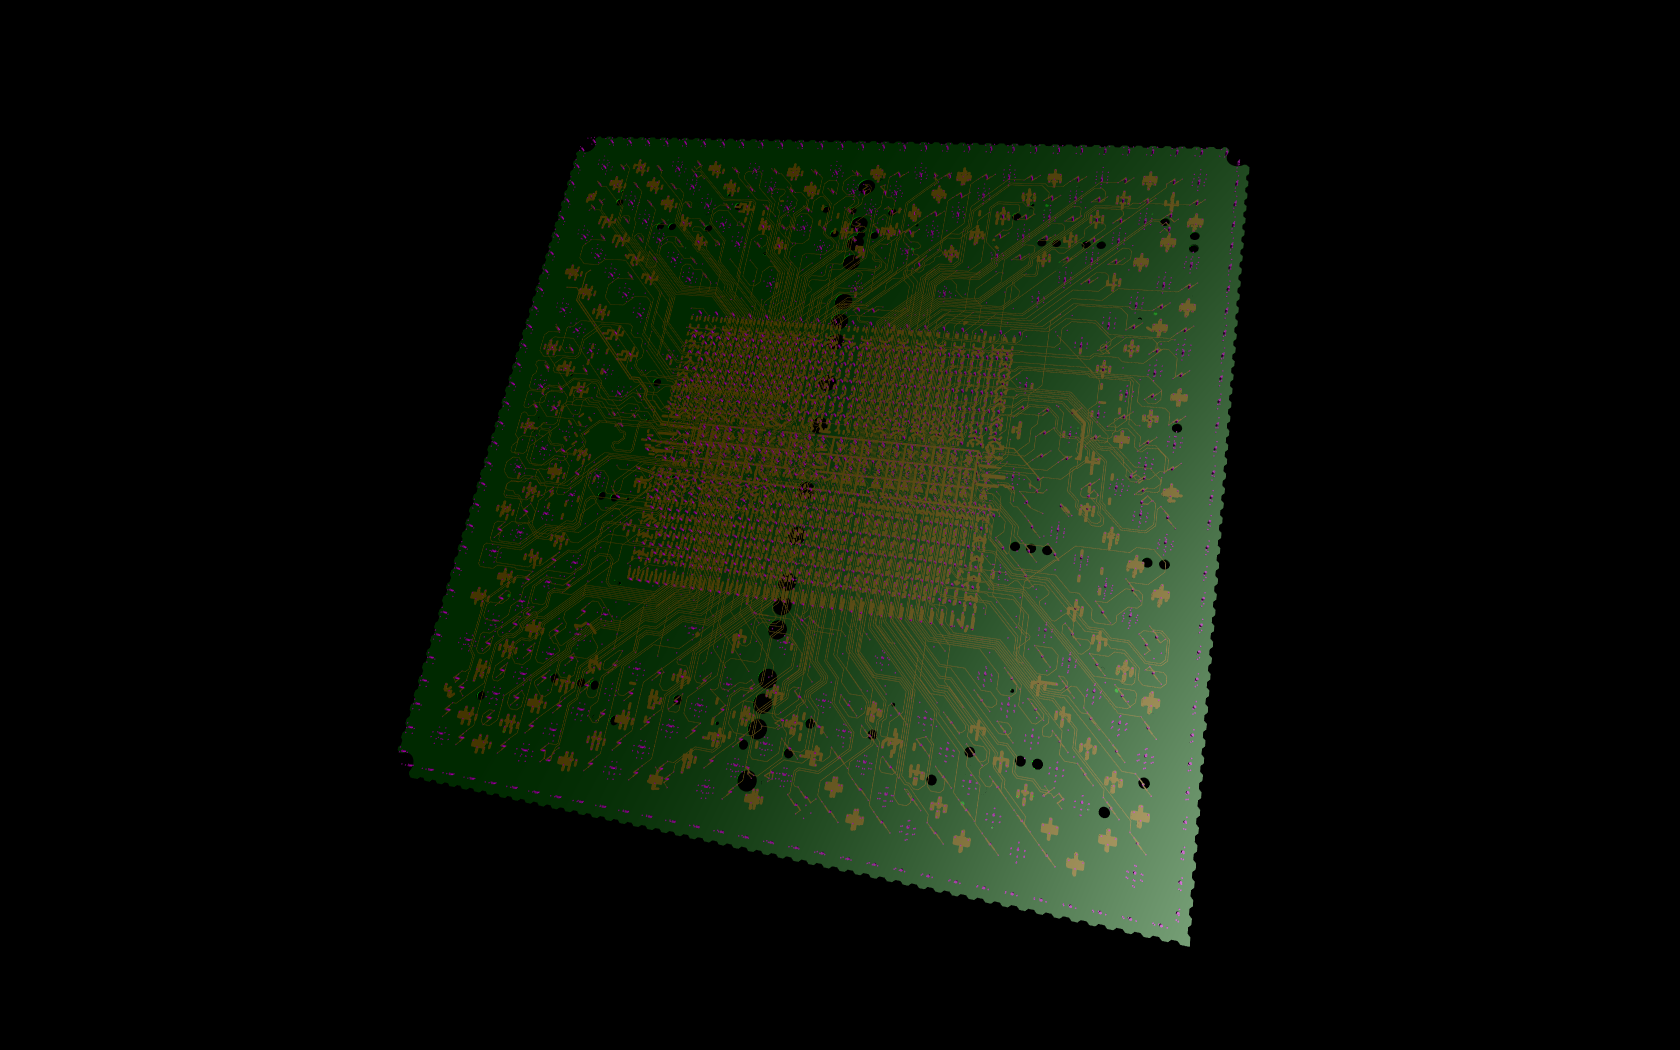
\includegraphics[width=0.45\linewidth]{figures/Plasma}
		}
		\subfigure{
			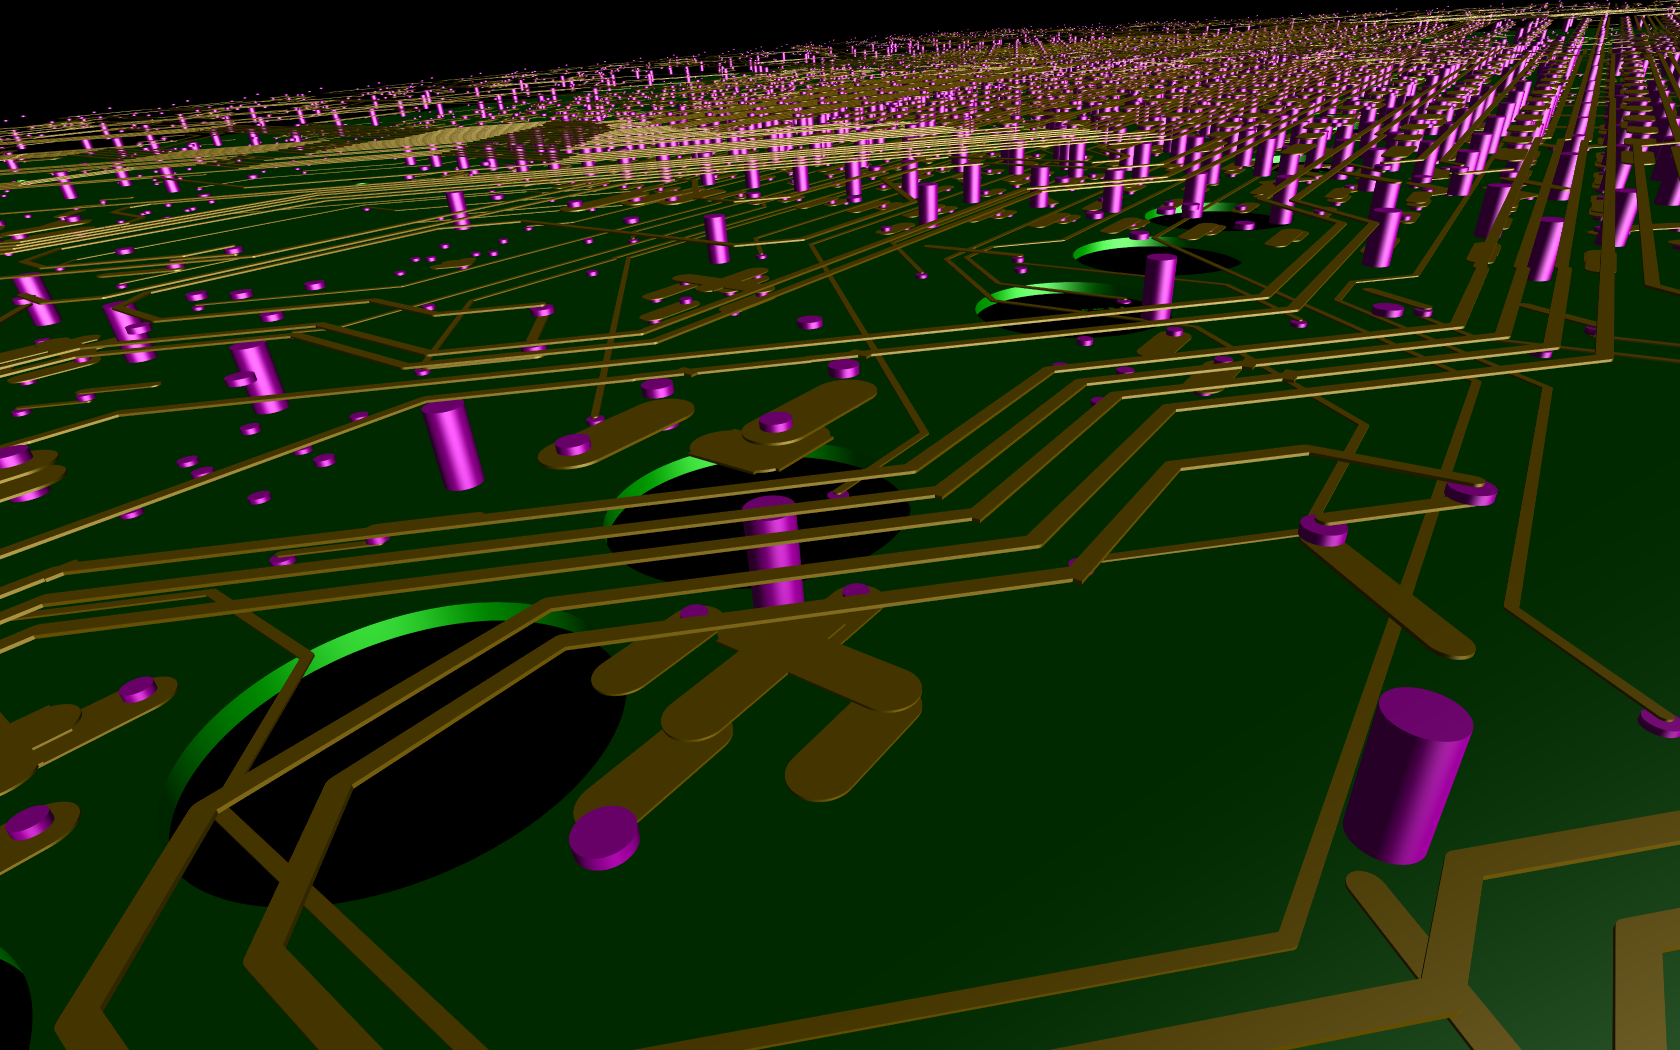
\includegraphics[width=0.45\linewidth]{figures/Plasma_Closeup}
		}\\
		\subfigure{
			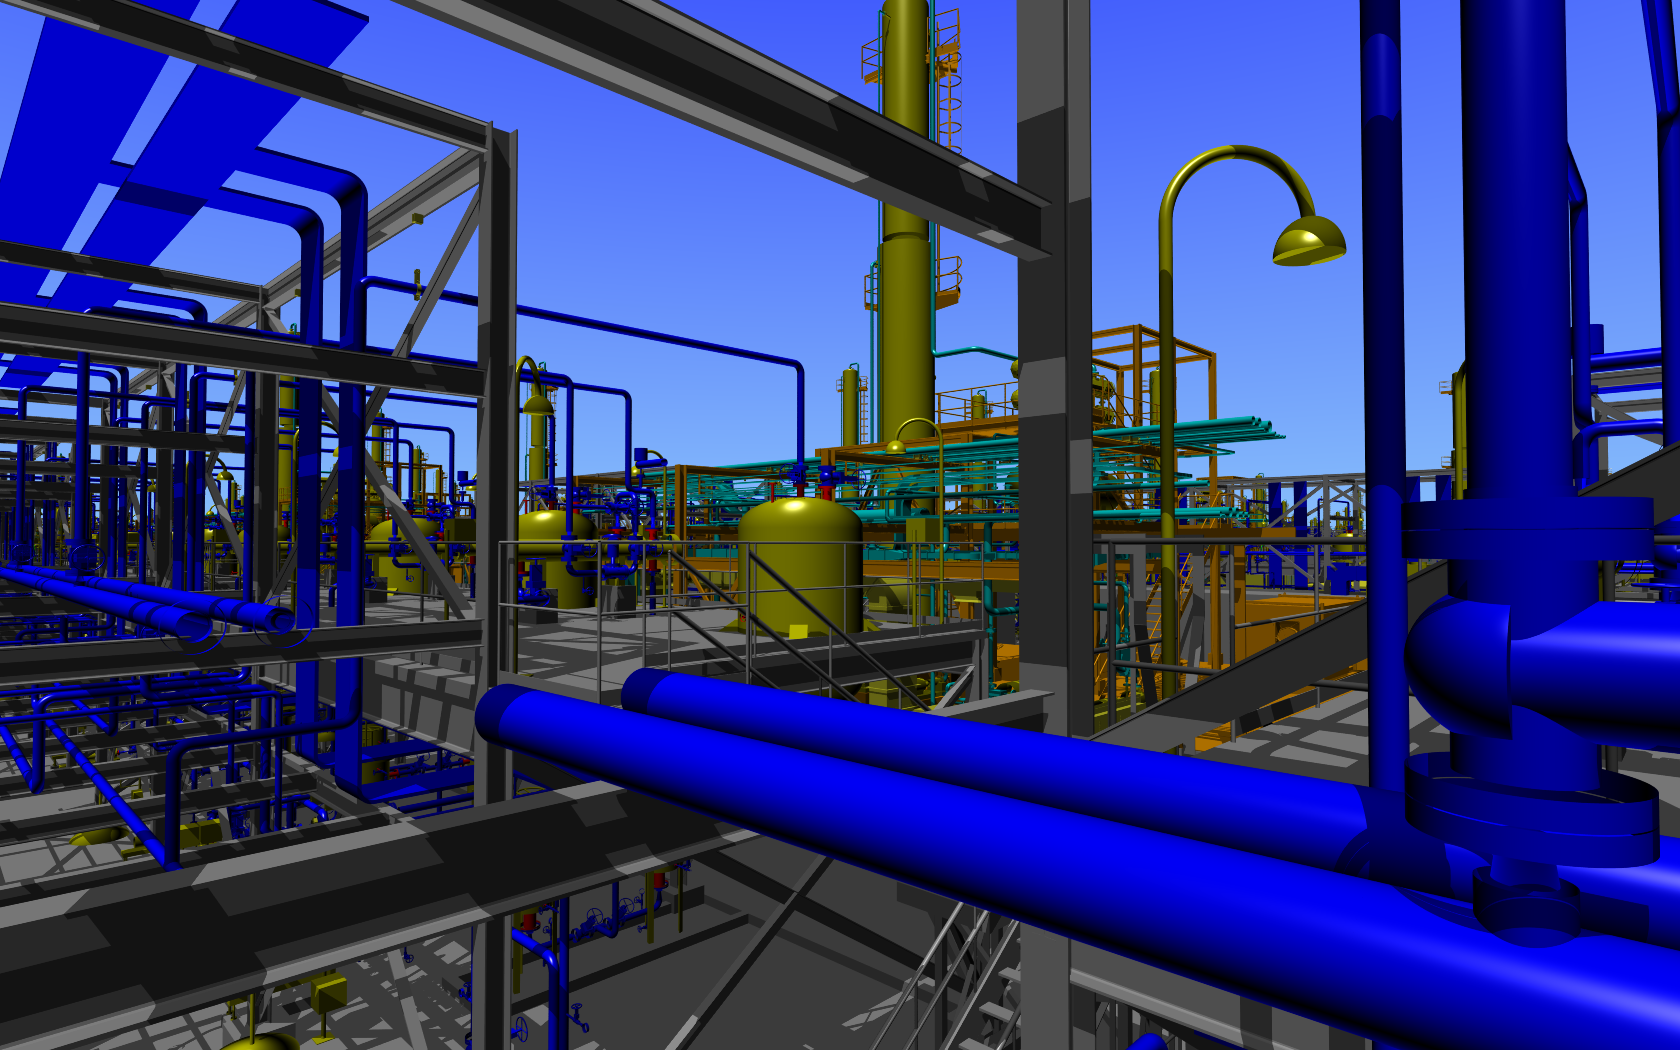
\includegraphics[width=0.45\linewidth]{figures/Plant_Closeup_1}
		}
		\subfigure{
			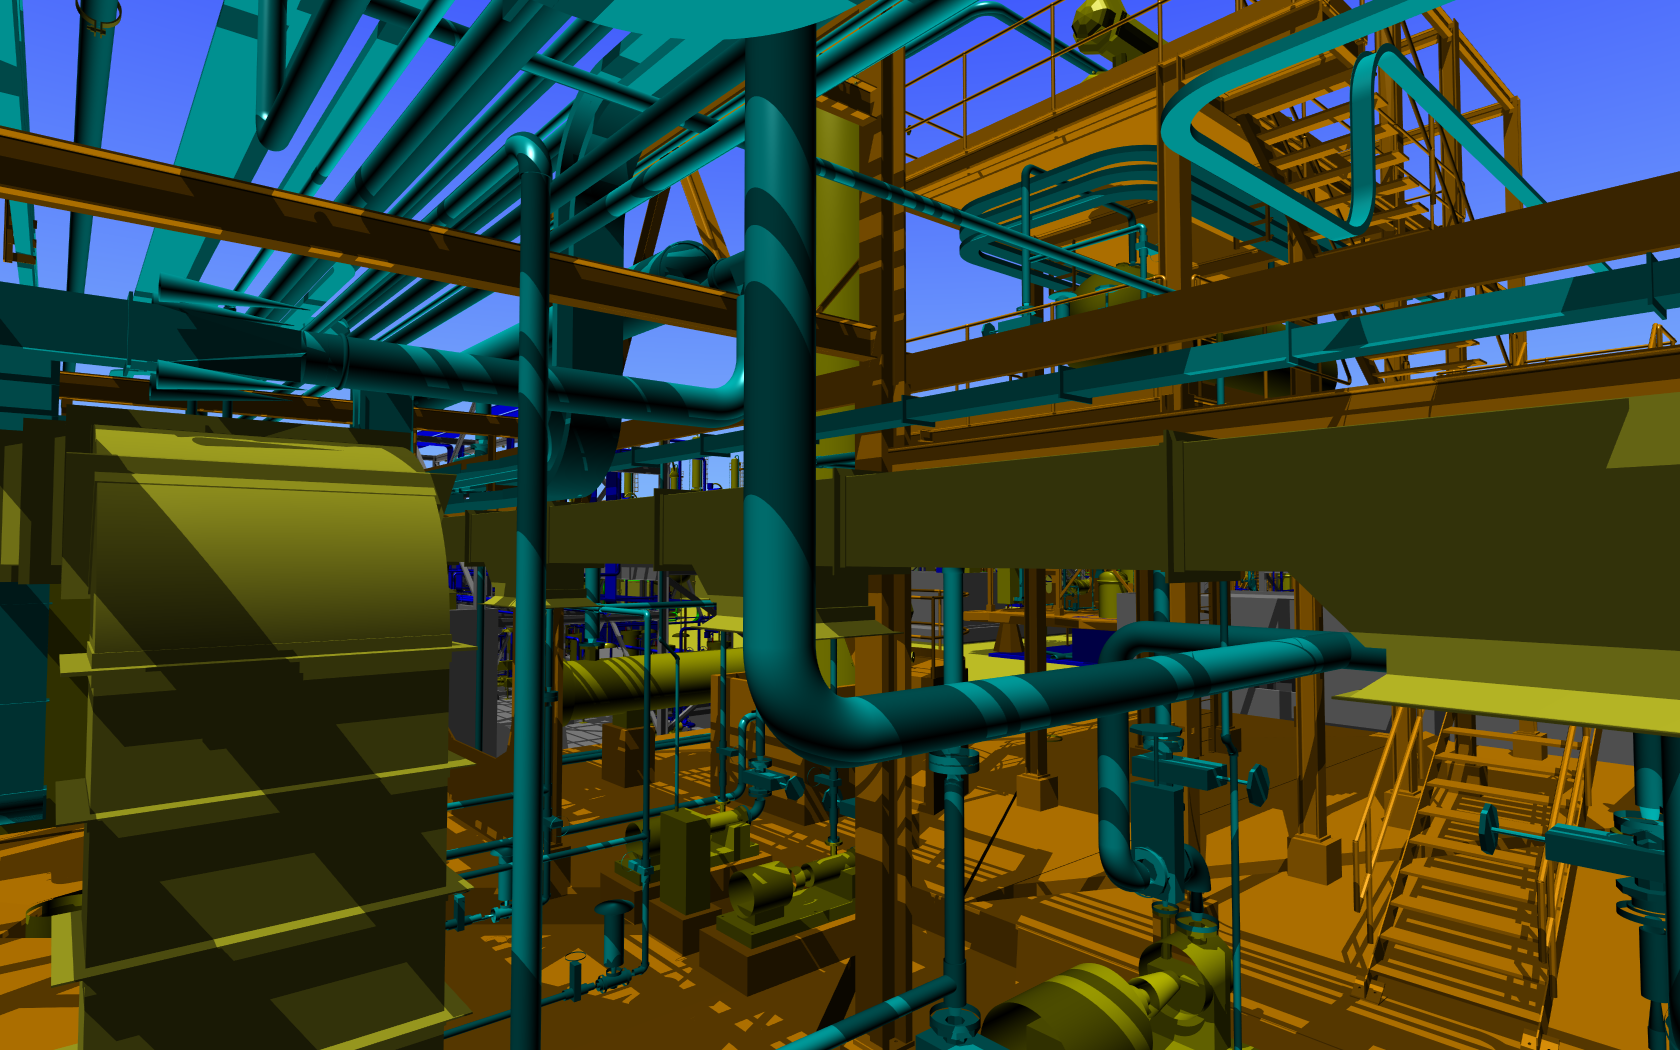
\includegraphics[width=0.45\linewidth]{figures/Plant_Closeup_2}
		}
	\end{figure}
\end{frame}

%================================================
%================================================

\section{Voxel based path tracing}

\begin{frame}{Outline}
	\tableofcontents
\end{frame}

\begin{frame}{Ray tracing revisited for rendering CSG models consisting of higher order primitives}
	\begin{figure}[ht!]
		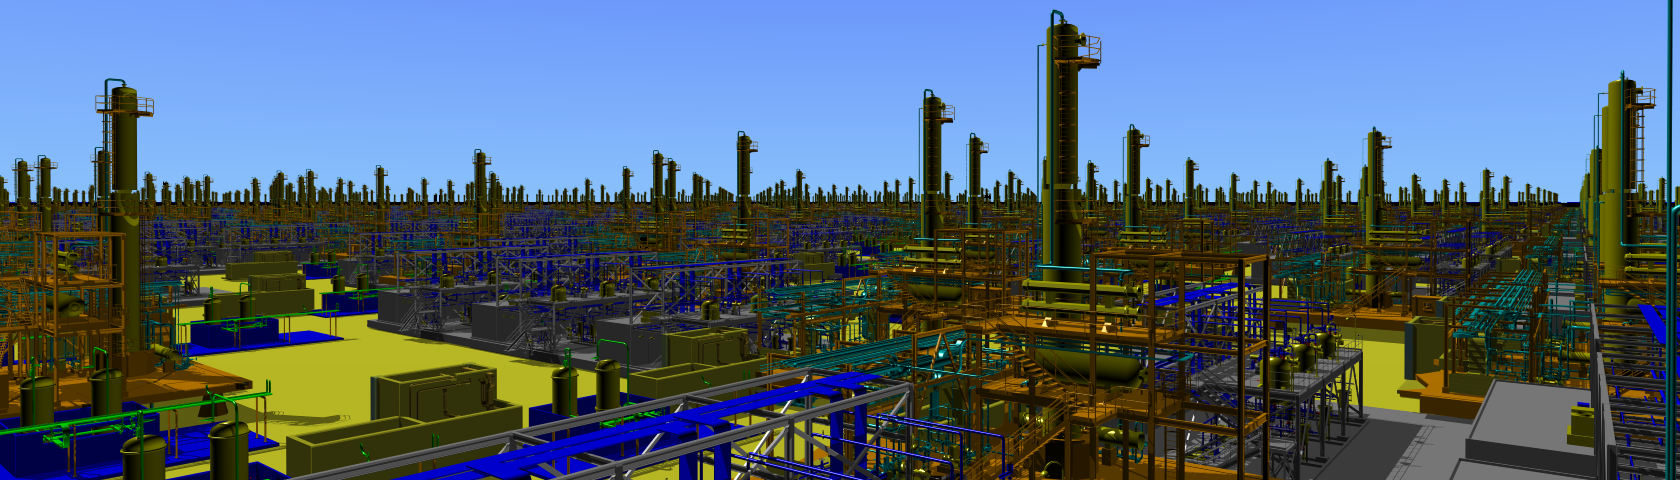
\includegraphics[width=1.0\linewidth]{figures/Plant_Teaser.png}
		\caption{
			A complex CAD scene built out of 8,000 individual plant models. In total, the scene consists of more than 100,000,000 non-planar second-order (cylinders, cones, etc.) and forth-order (tori) primitives, ray traced at more than 10~frames per second on 16 CPU
			cores, including pixel-accurate shadows.
		}
	\end{figure}
\end{frame}

%================================================
%================================================

\section{Other Projects}

\begin{frame}{Outline}
	\tableofcontents
\end{frame}


\begin{frame}{Practical Courses}
\end{frame}

\begin{frame}{Computer Graphics related courses}
\end{frame}

\begin{frame}{MetaIO}
\end{frame}

\begin{frame}{Zull Dutch}
\end{frame}

\begin{frame}{IDP}
\end{frame}

%================================================
%================================================

\section{Discussion}

\begin{frame}{Outline}
	\tableofcontents
\end{frame}

\begin{frame}{What do you want to be known for in next.}
\end{frame}

\begin{frame}[allowframebreaks]
	\frametitle{References}
	\bibliographystyle{amsalpha}
	\bibliography{bibliography}
\end{frame}


\end{document}